\documentclass[11pt]{article}

\usepackage{float}
% NOTE: Add in the relevant information to the commands below; or, if you'll be using the same information frequently, add these commands at the top of paolo-pset.tex file. 
\newcommand{\name}{Agustin Esteva}
\newcommand{\email}{aesteva@uchicago.edu}
\newcommand{\classnum}{13210}
\newcommand{\subject}{SSI: Formal Theory}
\newcommand{\instructors}{Scott Gehlbach}
\newcommand{\assignment}{Problem Set 2}
\newcommand{\semester}{Winter 2024}
\newcommand{\duedate}{2024-02-03}
\newcommand{\bA}{\mathbf{A}}
\newcommand{\bB}{\mathbf{B}}
\newcommand{\bC}{\mathbf{C}}
\newcommand{\bD}{\mathbf{D}}
\newcommand{\bE}{\mathbf{E}}
\newcommand{\bF}{\mathbf{F}}
\newcommand{\bG}{\mathbf{G}}
\newcommand{\bH}{\mathbf{H}}
\newcommand{\bI}{\mathbf{I}}
\newcommand{\bJ}{\mathbf{J}}
\newcommand{\bK}{\mathbf{K}}
\newcommand{\bL}{\mathbf{L}}
\newcommand{\bM}{\mathbf{M}}
\newcommand{\bN}{\mathbf{N}}
\newcommand{\bO}{\mathbf{O}}
\newcommand{\bP}{\mathbf{P}}
\newcommand{\bQ}{\mathbf{Q}}
\newcommand{\bR}{\mathbf{R}}
\newcommand{\bS}{\mathbf{S}}
\newcommand{\bT}{\mathbf{T}}
\newcommand{\bU}{\mathbf{U}}
\newcommand{\bV}{\mathbf{V}}
\newcommand{\bW}{\mathbf{W}}
\newcommand{\bX}{\mathbf{X}}
\newcommand{\bY}{\mathbf{Y}}
\newcommand{\bZ}{\mathbf{Z}}
\newcommand{\Var}{\text{Var}}

%% blackboard bold math capitals
\newcommand{\bbA}{\mathbb{A}}
\newcommand{\bbB}{\mathbb{B}}
\newcommand{\bbC}{\mathbb{C}}
\newcommand{\bbD}{\mathbb{D}}
\newcommand{\bbE}{\mathbb{E}}
\newcommand{\bbF}{\mathbb{F}}
\newcommand{\bbG}{\mathbb{G}}
\newcommand{\bbH}{\mathbb{H}}
\newcommand{\bbI}{\mathbb{I}}
\newcommand{\bbJ}{\mathbb{J}}
\newcommand{\bbK}{\mathbb{K}}
\newcommand{\bbL}{\mathbb{L}}
\newcommand{\bbM}{\mathbb{M}}
\newcommand{\bbN}{\mathbb{N}}
\newcommand{\bbO}{\mathbb{O}}
\newcommand{\bbP}{\mathbb{P}}
\newcommand{\bbQ}{\mathbb{Q}}
\newcommand{\bbR}{\mathbb{R}}
\newcommand{\bbS}{\mathbb{S}}
\newcommand{\bbT}{\mathbb{T}}
\newcommand{\bbU}{\mathbb{U}}
\newcommand{\bbV}{\mathbb{V}}
\newcommand{\bbW}{\mathbb{W}}
\newcommand{\bbX}{\mathbb{X}}
\newcommand{\bbY}{\mathbb{Y}}
\newcommand{\bbZ}{\mathbb{Z}}

%% script math capitals
\newcommand{\sA}{\mathscr{A}}
\newcommand{\sB}{\mathscr{B}}
\newcommand{\sC}{\mathscr{C}}
\newcommand{\sD}{\mathscr{D}}
\newcommand{\sE}{\mathscr{E}}
\newcommand{\sF}{\mathscr{F}}
\newcommand{\sG}{\mathscr{G}}
\newcommand{\sH}{\mathscr{H}}
\newcommand{\sI}{\mathscr{I}}
\newcommand{\sJ}{\mathscr{J}}
\newcommand{\sK}{\mathscr{K}}
\newcommand{\sL}{\mathscr{L}}
\newcommand{\sM}{\mathscr{M}}
\newcommand{\sN}{\mathscr{N}}
\newcommand{\sO}{\mathscr{O}}
\newcommand{\sP}{\mathscr{P}}
\newcommand{\sQ}{\mathscr{Q}}
\newcommand{\sR}{\mathscr{R}}
\newcommand{\sS}{\mathscr{S}}
\newcommand{\sT}{\mathscr{T}}
\newcommand{\sU}{\mathscr{U}}
\newcommand{\sV}{\mathscr{V}}
\newcommand{\sW}{\mathscr{W}}
\newcommand{\sX}{\mathscr{X}}
\newcommand{\sY}{\mathscr{Y}}
\newcommand{\sZ}{\mathscr{Z}}


\renewcommand{\emptyset}{\O}

\newcommand{\abs}[1]{\lvert #1 \rvert}
\newcommand{\norm}[1]{\lVert #1 \rVert}
\newcommand{\sm}{\setminus}


\newcommand{\sarr}{\rightarrow}
\newcommand{\arr}{\longrightarrow}

% NOTE: Defining collaborators is optional; to not list collaborators, comment out the line below.
%\newcommand{\collaborators}{Alyssa P. Hacker (\texttt{aphacker}), Ben Bitdiddle (\texttt{bitdiddle})}

% Copyright 2021 Paolo Adajar (padajar.com, paoloadajar@mit.edu)
% 
% Permission is hereby granted, free of charge, to any person obtaining a copy of this software and associated documentation files (the "Software"), to deal in the Software without restriction, including without limitation the rights to use, copy, modify, merge, publish, distribute, sublicense, and/or sell copies of the Software, and to permit persons to whom the Software is furnished to do so, subject to the following conditions:
%
% The above copyright notice and this permission notice shall be included in all copies or substantial portions of the Software.
% 
% THE SOFTWARE IS PROVIDED "AS IS", WITHOUT WARRANTY OF ANY KIND, EXPRESS OR IMPLIED, INCLUDING BUT NOT LIMITED TO THE WARRANTIES OF MERCHANTABILITY, FITNESS FOR A PARTICULAR PURPOSE AND NONINFRINGEMENT. IN NO EVENT SHALL THE AUTHORS OR COPYRIGHT HOLDERS BE LIABLE FOR ANY CLAIM, DAMAGES OR OTHER LIABILITY, WHETHER IN AN ACTION OF CONTRACT, TORT OR OTHERWISE, ARISING FROM, OUT OF OR IN CONNECTION WITH THE SOFTWARE OR THE USE OR OTHER DEALINGS IN THE SOFTWARE.

\usepackage{fullpage}
\usepackage{enumitem}
\usepackage{amsfonts, amssymb, amsmath,amsthm}
\usepackage{mathtools}
\usepackage[pdftex, pdfauthor={\name}, pdftitle={\classnum~\assignment}]{hyperref}
\usepackage[dvipsnames]{xcolor}
\usepackage{bbm}
\usepackage{graphicx}
\usepackage{mathrsfs}
\usepackage{pdfpages}
\usepackage{tabularx}
\usepackage{pdflscape}
\usepackage{makecell}
\usepackage{booktabs}
\usepackage{natbib}
\usepackage{caption}
\usepackage{subcaption}
\usepackage{physics}
\usepackage[many]{tcolorbox}
\usepackage{version}
\usepackage{ifthen}
\usepackage{cancel}
\usepackage{listings}
\usepackage{courier}

\usepackage{tikz}
\usepackage{istgame}

\hypersetup{
	colorlinks=true,
	linkcolor=blue,
	filecolor=magenta,
	urlcolor=blue,
}

\setlength{\parindent}{0mm}
\setlength{\parskip}{2mm}

\setlist[enumerate]{label=({\alph*})}
\setlist[enumerate, 2]{label=({\roman*})}

\allowdisplaybreaks[1]

\newcommand{\psetheader}{
	\ifthenelse{\isundefined{\collaborators}}{
		\begin{center}
			{\setlength{\parindent}{0cm} \setlength{\parskip}{0mm}
				
				{\textbf{\classnum~\semester:~\assignment} \hfill \name}
				
				\subject \hfill \href{mailto:\email}{\tt \email}
				
				Instructor(s):~\instructors \hfill Due Date:~\duedate	
				
				\hrulefill}
		\end{center}
	}{
		\begin{center}
			{\setlength{\parindent}{0cm} \setlength{\parskip}{0mm}
				
				{\textbf{\classnum~\semester:~\assignment} \hfill \name\footnote{Collaborator(s): \collaborators}}
				
				\subject \hfill \href{mailto:\email}{\tt \email}
				
				Instructor(s):~\instructors \hfill Due Date:~\duedate	
				
				\hrulefill}
		\end{center}
	}
}

\renewcommand{\thepage}{\classnum~\assignment \hfill \arabic{page}}

\makeatletter
\def\points{\@ifnextchar[{\@with}{\@without}}
\def\@with[#1]#2{{\ifthenelse{\equal{#2}{1}}{{[1 point, #1]}}{{[#2 points, #1]}}}}
\def\@without#1{\ifthenelse{\equal{#1}{1}}{{[1 point]}}{{[#1 points]}}}
\makeatother

\newtheoremstyle{theorem-custom}%
{}{}%
{}{}%
{\itshape}{.}%
{ }%
{\thmname{#1}\thmnumber{ #2}\thmnote{ (#3)}}

\theoremstyle{theorem-custom}

\newtheorem{theorem}{Theorem}
\newtheorem{lemma}[theorem]{Lemma}
\newtheorem{example}[theorem]{Example}

\newenvironment{problem}[1]{\color{black} #1}{}

\newenvironment{solution}{%
	\leavevmode\begin{tcolorbox}[breakable, colback=green!5!white,colframe=green!75!black, enhanced jigsaw] \proof[\scshape Solution:] \setlength{\parskip}{2mm}%
	}{\renewcommand{\qedsymbol}{$\blacksquare$} \endproof \end{tcolorbox}}

\newenvironment{reflection}{\begin{tcolorbox}[breakable, colback=black!8!white,colframe=black!60!white, enhanced jigsaw, parbox = false]\textsc{Reflections:}}{\end{tcolorbox}}

\newcommand{\qedh}{\renewcommand{\qedsymbol}{$\blacksquare$}\qedhere}

\definecolor{mygreen}{rgb}{0,0.6,0}
\definecolor{mygray}{rgb}{0.5,0.5,0.5}
\definecolor{mymauve}{rgb}{0.58,0,0.82}

% from https://github.com/satejsoman/stata-lstlisting
% language definition
\lstdefinelanguage{Stata}{
	% System commands
	morekeywords=[1]{regress, reg, summarize, sum, display, di, generate, gen, bysort, use, import, delimited, predict, quietly, probit, margins, test},
	% Reserved words
	morekeywords=[2]{aggregate, array, boolean, break, byte, case, catch, class, colvector, complex, const, continue, default, delegate, delete, do, double, else, eltypedef, end, enum, explicit, export, external, float, for, friend, function, global, goto, if, inline, int, local, long, mata, matrix, namespace, new, numeric, NULL, operator, orgtypedef, pointer, polymorphic, pragma, private, protected, public, quad, real, return, rowvector, scalar, short, signed, static, strL, string, struct, super, switch, template, this, throw, transmorphic, try, typedef, typename, union, unsigned, using, vector, version, virtual, void, volatile, while,},
	% Keywords
	morekeywords=[3]{forvalues, foreach, set},
	% Date and time functions
	morekeywords=[4]{bofd, Cdhms, Chms, Clock, clock, Cmdyhms, Cofc, cofC, Cofd, cofd, daily, date, day, dhms, dofb, dofC, dofc, dofh, dofm, dofq, dofw, dofy, dow, doy, halfyear, halfyearly, hh, hhC, hms, hofd, hours, mdy, mdyhms, minutes, mm, mmC, mofd, month, monthly, msofhours, msofminutes, msofseconds, qofd, quarter, quarterly, seconds, ss, ssC, tC, tc, td, th, tm, tq, tw, week, weekly, wofd, year, yearly, yh, ym, yofd, yq, yw,},
	% Mathematical functions
	morekeywords=[5]{abs, ceil, cloglog, comb, digamma, exp, expm1, floor, int, invcloglog, invlogit, ln, ln1m, ln, ln1p, ln, lnfactorial, lngamma, log, log10, log1m, log1p, logit, max, min, mod, reldif, round, sign, sqrt, sum, trigamma, trunc,},
	% Matrix functions
	morekeywords=[6]{cholesky, coleqnumb, colnfreeparms, colnumb, colsof, corr, det, diag, diag0cnt, el, get, hadamard, I, inv, invsym, issymmetric, J, matmissing, matuniform, mreldif, nullmat, roweqnumb, rownfreeparms, rownumb, rowsof, sweep, trace, vec, vecdiag, },
	% Programming functions
	morekeywords=[7]{autocode, byteorder, c, _caller, chop, abs, clip, cond, e, fileexists, fileread, filereaderror, filewrite, float, fmtwidth, has_eprop, inlist, inrange, irecode, matrix, maxbyte, maxdouble, maxfloat, maxint, maxlong, mi, minbyte, mindouble, minfloat, minint, minlong, missing, r, recode, replay, return, s, scalar, smallestdouble,},
	% Random-number functions
	morekeywords=[8]{rbeta, rbinomial, rcauchy, rchi2, rexponential, rgamma, rhypergeometric, rigaussian, rlaplace, rlogistic, rnbinomial, rnormal, rpoisson, rt, runiform, runiformint, rweibull, rweibullph,},
	% Selecting time-span functions
	morekeywords=[9]{tin, twithin,},
	% Statistical functions
	morekeywords=[10]{betaden, binomial, binomialp, binomialtail, binormal, cauchy, cauchyden, cauchytail, chi2, chi2den, chi2tail, dgammapda, dgammapdada, dgammapdadx, dgammapdx, dgammapdxdx, dunnettprob, exponential, exponentialden, exponentialtail, F, Fden, Ftail, gammaden, gammap, gammaptail, hypergeometric, hypergeometricp, ibeta, ibetatail, igaussian, igaussianden, igaussiantail, invbinomial, invbinomialtail, invcauchy, invcauchytail, invchi2, invchi2tail, invdunnettprob, invexponential, invexponentialtail, invF, invFtail, invgammap, invgammaptail, invibeta, invibetatail, invigaussian, invigaussiantail, invlaplace, invlaplacetail, invlogistic, invlogistictail, invnbinomial, invnbinomialtail, invnchi2, invnF, invnFtail, invnibeta, invnormal, invnt, invnttail, invpoisson, invpoissontail, invt, invttail, invtukeyprob, invweibull, invweibullph, invweibullphtail, invweibulltail, laplace, laplaceden, laplacetail, lncauchyden, lnigammaden, lnigaussianden, lniwishartden, lnlaplaceden, lnmvnormalden, lnnormal, lnnormalden, lnwishartden, logistic, logisticden, logistictail, nbetaden, nbinomial, nbinomialp, nbinomialtail, nchi2, nchi2den, nchi2tail, nF, nFden, nFtail, nibeta, normal, normalden, npnchi2, npnF, npnt, nt, ntden, nttail, poisson, poissonp, poissontail, t, tden, ttail, tukeyprob, weibull, weibullden, weibullph, weibullphden, weibullphtail, weibulltail,},
	% String functions 
	morekeywords=[11]{abbrev, char, collatorlocale, collatorversion, indexnot, plural, plural, real, regexm, regexr, regexs, soundex, soundex_nara, strcat, strdup, string, strofreal, string, strofreal, stritrim, strlen, strlower, strltrim, strmatch, strofreal, strofreal, strpos, strproper, strreverse, strrpos, strrtrim, strtoname, strtrim, strupper, subinstr, subinword, substr, tobytes, uchar, udstrlen, udsubstr, uisdigit, uisletter, ustrcompare, ustrcompareex, ustrfix, ustrfrom, ustrinvalidcnt, ustrleft, ustrlen, ustrlower, ustrltrim, ustrnormalize, ustrpos, ustrregexm, ustrregexra, ustrregexrf, ustrregexs, ustrreverse, ustrright, ustrrpos, ustrrtrim, ustrsortkey, ustrsortkeyex, ustrtitle, ustrto, ustrtohex, ustrtoname, ustrtrim, ustrunescape, ustrupper, ustrword, ustrwordcount, usubinstr, usubstr, word, wordbreaklocale, worcount,},
	% Trig functions
	morekeywords=[12]{acos, acosh, asin, asinh, atan, atanh, cos, cosh, sin, sinh, tan, tanh,},
	morecomment=[l]{//},
	% morecomment=[l]{*},  // `*` maybe used as multiply operator. So use `//` as line comment.
	morecomment=[s]{/*}{*/},
	% The following is used by macros, like `lags'.
	morestring=[b]{`}{'},
	% morestring=[d]{'},
	morestring=[b]",
	morestring=[d]",
	% morestring=[d]{\\`},
	% morestring=[b]{'},
	sensitive=true,
}

\lstset{ 
	backgroundcolor=\color{white},   % choose the background color; you must add \usepackage{color} or \usepackage{xcolor}; should come as last argument
	basicstyle=\footnotesize\ttfamily,        % the size of the fonts that are used for the code
	breakatwhitespace=false,         % sets if automatic breaks should only happen at whitespace
	breaklines=true,                 % sets automatic line breaking
	captionpos=b,                    % sets the caption-position to bottom
	commentstyle=\color{mygreen},    % comment style
	deletekeywords={...},            % if you want to delete keywords from the given language
	escapeinside={\%*}{*)},          % if you want to add LaTeX within your code
	extendedchars=true,              % lets you use non-ASCII characters; for 8-bits encodings only, does not work with UTF-8
	firstnumber=0,                % start line enumeration with line 1000
	frame=single,	                   % adds a frame around the code
	keepspaces=true,                 % keeps spaces in text, useful for keeping indentation of code (possibly needs columns=flexible)
	keywordstyle=\color{blue},       % keyword style
	language=Octave,                 % the language of the code
	morekeywords={*,...},            % if you want to add more keywords to the set
	numbers=left,                    % where to put the line-numbers; possible values are (none, left, right)
	numbersep=5pt,                   % how far the line-numbers are from the code
	numberstyle=\tiny\color{mygray}, % the style that is used for the line-numbers
	rulecolor=\color{black},         % if not set, the frame-color may be changed on line-breaks within not-black text (e.g. comments (green here))
	showspaces=false,                % show spaces everywhere adding particular underscores; it overrides 'showstringspaces'
	showstringspaces=false,          % underline spaces within strings only
	showtabs=false,                  % show tabs within strings adding particular underscores
	stepnumber=2,                    % the step between two line-numbers. If it's 1, each line will be numbered
	stringstyle=\color{mymauve},     % string literal style
	tabsize=2,	                   % sets default tabsize to 2 spaces
%	title=\lstname,                   % show the filename of files included with \lstinputlisting; also try caption instead of title
	xleftmargin=0.25cm
}

% NOTE: To compile a version of this pset without problems, solutions, or reflections, uncomment the relevant line below.

%\excludeversion{problem}
%\excludeversion{solution}
%\excludeversion{reflection}

\begin{document}	
	
	% Use the \psetheader command at the beginning of a pset. 
	\psetheader
\section*{Problem 1}

\begin{problem}
Are the following two strategic games with von Neumann-Morgenstern preferences equivalent? Why or why not?
    

\[
    \begin{array}{c|cc}
        & O & B \\
        \hline
        O & 2, 1 & 0, 0 \\
        B & 0, 0 & 1, 2 \\
    \end{array}
    \quad
    \begin{array}{c|cc}
        & O & B \\
        \hline
        O & 1.25, -3.2 & -3.2, -1.3 \\
        B & -3.2, -1.3 & 1.2, 1.2 \\
    \end{array}
    \]
    
\end{problem}
\begin{solution}
    No.  On the table on the left, player $1$'s payoff to (B,B) is the same as the expected payoff to the lottery that yields $(O,O)$ with probability $\frac{1}{2}$ and $(O,B)$ with probability $\frac{1}{2}$ since
    \[\alpha_1(O) = \frac{1}{2}u_1(O,O) + \frac{1}{2}u_1(O,F) = 1\]
    \[\alpha'_1(B) = 0u_1(B,O) + 1u_1(B,B) = 1\]
    But in the second game, we have that 
    \[\alpha_1(O) = \frac{1}{2}u_1(O,O) + \frac{1}{2}u_1(O,B) = -.975\]
    \[\alpha'_1(B) = 0 u_1(B,O) + 1 u_1(B,B) = 1.2.\] Thus, we have that while in the first table, player $1$ is indifferent between a deterministic outcome of $(B,B)$ and a lottery, we have that in the second table, player $1$ prefers a lottery to a deterministic outcome $(B,B).$ This is a different way of seeing that vNM tables are not equivalent. 

    For the usual affine transformation way, suppose they are equivalent, then any utility in the second table can be expressed as $u_2 = au_1 + b.$ We see that $b = -3.2$ since $u_2 = au_1(O,B) + b = 0 + b = -3.2,$ but then $1.25 = au_2(O,O) - 3.2 = 2a - 3.2 \implies a = 2.225$ which is a contradiction since $1.2 = u_2(B,B) \neq 2.225 - 3.2$
\end{solution}



\newpage
\section*{Problem 2}

\begin{problem}
Kahneman and Tversky find that $b$ and $c$ are the modal choices in the following experiment:
    \begin{itemize}
        \item Treatment 1: A person has been given \$1000 and offered the choice of:
        \begin{itemize}
            \item Lottery $a$: 0.5 chance of an additional \$1000, 0.5 chance of no change in the endowment
            \item Lottery $b$: An additional \$500 for sure
        \end{itemize}
        \item Treatment 2: A person has been given \$2000 and offered the choice of:
        \begin{itemize}
            \item Lottery $c$: 0.5 chance of losing \$1000, 0.5 chance of no change in the endowment
            \item Lottery $d$: Losing \$500 for sure
        \end{itemize}
    \end{itemize}
    Are these choices consistent with von Neumann-Morgenstern preferences over lotteries over outcomes? Why or why not?
    
\end{problem}
\begin{solution}
    Suppose they are consistent, then since people prefer $a$ to $b,$ we have that 
    \[\frac{1}{2}u(2) + \frac{1}{2}u(1) < 1u(1.5)\] and since people prefer $c$ to $d,$ we have that
    \[\frac{1}{2}u(1) + \frac{1}{2}u(2) > 1u(1.5).\] Then chaining these equalities together
    \[\frac{1}{2}u(1) + \frac{1}{2}u(2) > \frac{1}{2}u(2) + \frac{1}{2}u(1),\] which is a contradiction, since these are obviously equal!
\end{solution}

\newpage
\section*{Problem 3}
\begin{problem}
For the following games, derive the best response for each player and find all mixed-strategy Nash equilibria.
    \begin{enumerate}
        \item 
        

\[
        \begin{array}{c|cc}
            & \text{Left} & \text{Right} \\
            \hline
            \text{Up} & -5, -5 & x - 15, 0 \\
            \text{Down} & 0, 15 & 10, 10 \\
        \end{array}
        \quad \text{where } x < 25
        \]
\begin{solution}
    Obviously, $(D,L)$ is a Nash Equilibrium and so the pure strategy of $(p, q) = (0,1)$ is a Nash Equilibrium. 
    
    For player 1: Consider that 
    \[u_1(U, q) = -5q + (x-15)(1-q)\]
    \[u_1(D,q) = 0q + 10(1-q) = 10 - 10q\] and so 
    \[q' = \frac{x- 25}{x-20} \implies u_1(U, q')= u_1(D, q').\] Thus, since $q <0<q'$ for all $x<25,$ we have that $u_1(D) > u_1(U)$ for any $q,$ and so player $1$ chooses $p = 0$ for any $q$ (he always goes down). 

    For player 2:
    \[u_2(L, p) = -5p + 15(1-p)\]
    \[u_2(R, p) = 0p + 10(1-p),\]
    and so 
    \[p' = \frac{1}{2} \implies u_1(L, p')= u_1(R, p'),\] and if $p< p',$ we have that player two goes left, ($q = 1$) and if $p>p',$ we have that player two goes right ($q = 0$). 

    Thus, we only have a single Nash equilibrium since the best responses coincide only at $((p^*, q^*) = (0,1) = (D,L).$
\end{solution}

        \item 
        

\[
        \begin{array}{c|cc}
            & \text{Left} & \text{Right} \\
            \hline
            \text{Up} & -5, -5 & x - 15, 0 \\
            \text{Down} & 0, 15 & 10, 10 \\
        \end{array}
        \quad \text{where } x = 25
        \]


    
\begin{solution}
    We see from above that if $x = 25,$ then $q' = 0 \implies u_1(U,q') = u_1(D, q').$ Thus, player $1$ chooses $p=1$ if $q=0$ since this guarantees that $u_1(U)\geq u_1(U).$ If $q>0,$ we see that $p=0$ since $u_1(U,q)< u_1(D,q).$ From above, and from the best response graph below, we see that this will intersect the best response at the points::
    \[(p^*, q^*) = \{(0,1), ([\frac{1}{2},1], 0\}.\]
\end{solution}

\item 
\begin{problem}
    Same game where $x>25.$
\end{problem}
\begin{solution}
    We see that if $q< \frac{x-25}{x-20},$ then $p = 1$ and if $q>\frac{x-25}{x-20},$ then $p = 0.$ Thus, we have three equilibrium, $(0,1), (1,0)$, and a new one at
    \[(p,q) = (\frac{1}{2}, \frac{x-25}{x-20}).\]
\end{solution}
    \end{enumerate}
\begin{figure}[H]
    \centering
    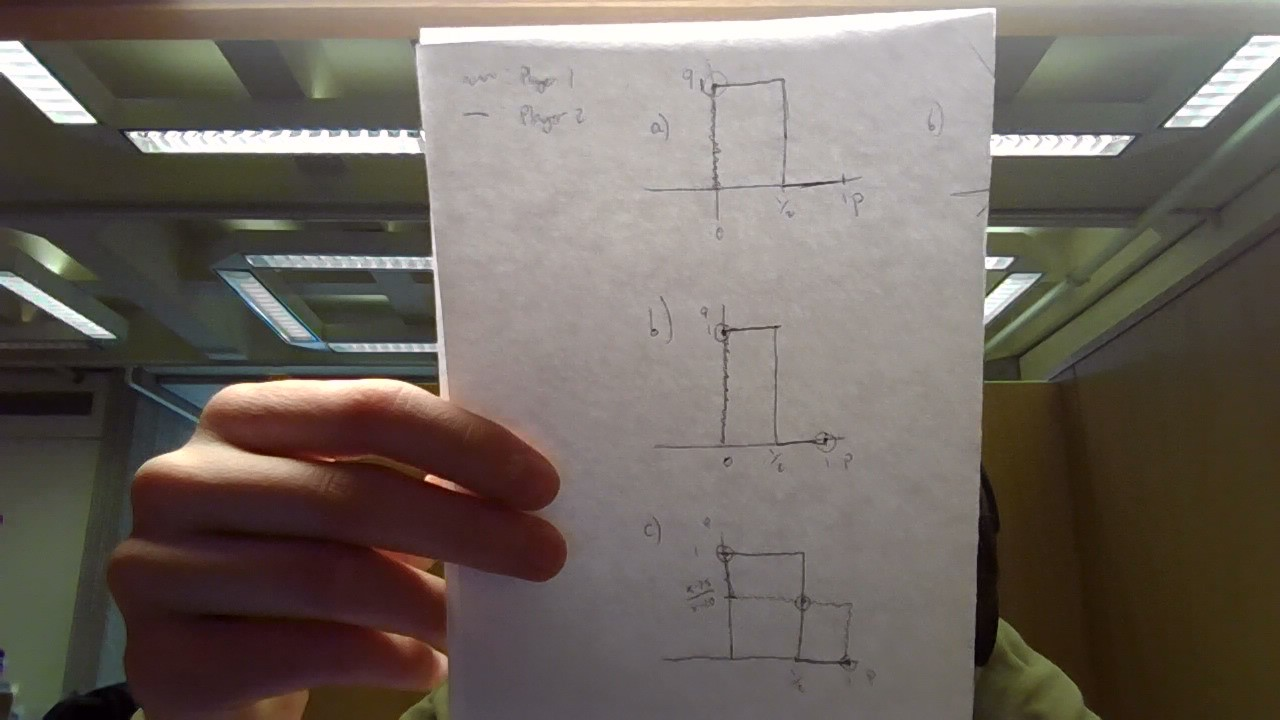
\includegraphics[width=0.5\linewidth]{Images/WIN_20250216_16_09_31_Pro.jpg}
    \caption{Best Response Functions for Above Problems}
\end{figure}
\end{problem}

\newpage
\section*{Problem 4}
\begin{problem}
\begin{tabular}{c|cc}
    & \text{Swerve} & \text{Straight} \\
    \hline
    \text{Swerve} & 0,0 & -1,1 \\
    \text{Straight} & 1,-1 & -10,-10 \\
\end{tabular}
\begin{enumerate}
    \item Derive the best response for each player, marking clearly in a graph of the two best responses which best response belongs to player 1, and which to player 2.
\begin{solution}
    We have that 
    \[u_1(Sw) = 0q + (-1)(1-q) = -1 + q\]
    \[u_2(St) = 1(q) + (-10)(1-q) = -10 + 11q\]
    Thus, we have that 
    \[q' = \frac{9}{10} \implies u_1(Sw) = u_1(St),\] and so if $q< \frac{9}{10},$ then $u_1(Sw) > u_1(St)$ and so $p = 1$ and if $q>\frac{9}{10},$ then $p = 0.$ By symmetry, we have that if 
    \[p< \frac{9}{10}\implies q = 1, \qquad p>\frac{9}{10} \implies q = 0.\]
\end{solution}
\begin{figure}[H]
    \centering
    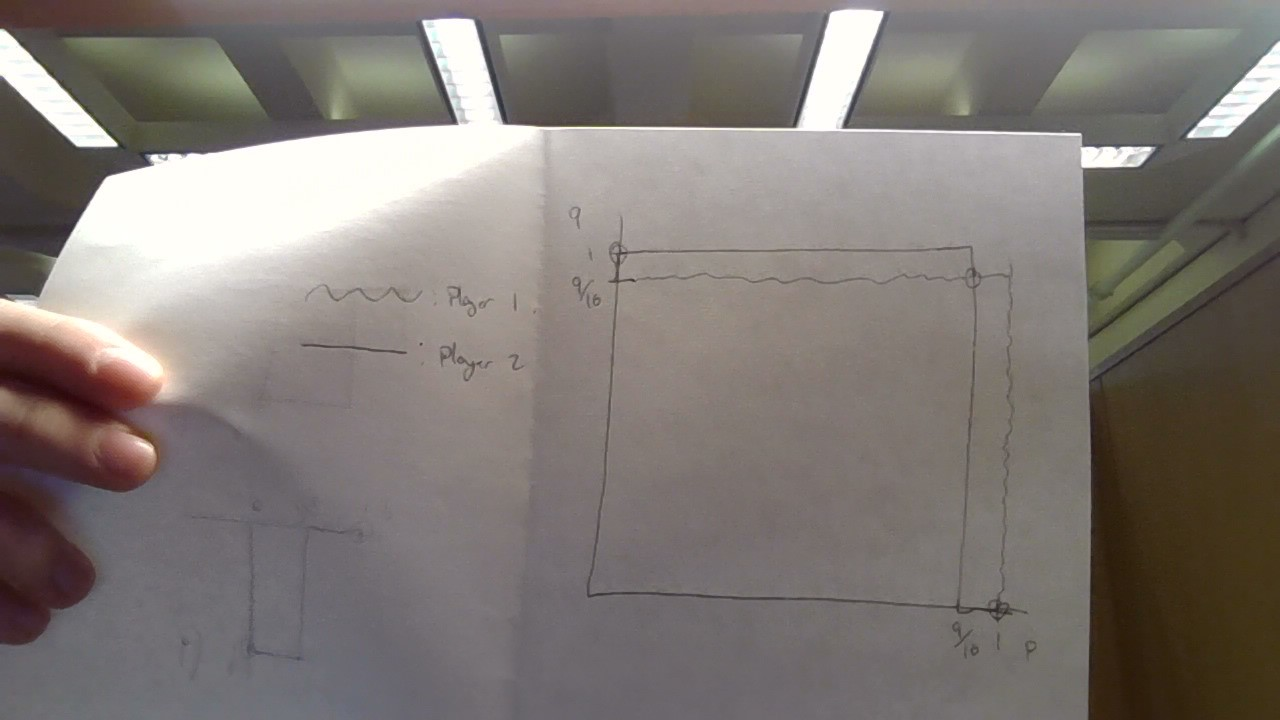
\includegraphics[width=0.75\linewidth]{WIN_20250216_16_15_13_Pro.jpg}
    \caption{Best Response Functions}
\end{figure}
    \item Find the set of mixed-strategy Nash equilibria.
    \begin{solution}
        From the best response functions above, we see intersections at the Nash equilibria of:
        \[(p^*, q^*) = \{(0,1), (\frac{9}{10}, \frac{9}{10}), (1,0)\}\]
    \end{solution}
    \item Which, if any, equilibria do you find compelling as a prediction for behavior in the strategic environment modeled by this game (two status-conscious but reckless teenagers barreling down the road toward each other)?
    \end{enumerate}
    \begin{solution}
        In the long run, I actually think that the mixed strategy makes sense to me. Assuming these are indestructible teenagers who feel pain, it makes sense that they would each swerve, on average, nine out of ten times. 
    \end{solution}
\end{problem}






\end{document}